%
% File acl2012.tex
%
% Contact: Maggie Li (cswjli@comp.polyu.edu.hk), Michael White (mwhite@ling.osu.edu)
%%
%% Based on the style files for ACL2008 by Joakim Nivre and Noah Smith
%% and that of ACL2010 by Jing-Shin Chang and Philipp Koehn


\documentclass[11pt,letterpaper]{article}
\usepackage[letterpaper]{geometry}
\usepackage{acl2012}
\usepackage{times}
\usepackage{latexsym}
\usepackage{amsmath}
\usepackage{multirow}
\usepackage{graphicx}
\usepackage{url}
\makeatletter
\newcommand{\@BIBLABEL}{\@emptybiblabel}
\newcommand{\@emptybiblabel}[1]{}
\makeatother
\usepackage[hidelinks]{hyperref}
\DeclareMathOperator*{\argmax}{arg\,max}
\setlength\titlebox{6.5cm}    % Expanding the titlebox

\title{Neural and Symbolic Arabic Paraphasing with Automatic Evaluation}

\author{First Author \\
  Affiliation / Address line 1 \\
  Affiliation / Address line 2 \\
  Affiliation / Address line 3 \\
  {\tt email@domain} \\\And
  Second Author \\
  Affiliation / Address line 1 \\
  Affiliation / Address line 2 \\
  Affiliation / Address line 3 \\
  {\tt email@domain} \\}

\date{}

\begin{document}
\maketitle
\begin{abstract}
We present a tool for Arabic paraphrasing that yields good paraphrasing accuracy.  We present and compare several methods for paraphrasing and obtaining monolingual parallel data. We also present first results on Arabic paraphrasing using neural methods. Additionally, we propose a new evaluation metric for paraphrasing that is shown to correlate highly with human judgement.
\end{abstract}


\section{Introduction}

\section{Related Work}

\section{Obtaining Parallel Monolingual Data}

\section{Extracting Paraphases}
In order to extract paraphrases, we first obtained a parallel bilingual corpus using the EUROPARL dataset \cite{Koehn_europarl}. \cite{bannard2005bilingual}
\begin{figure*}
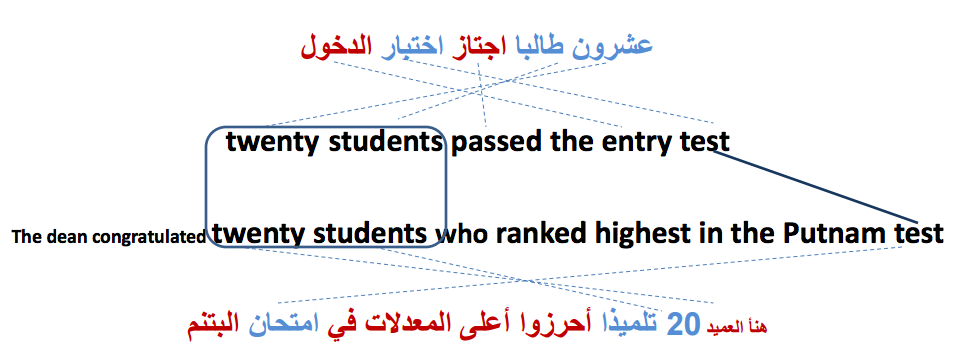
\includegraphics[scale=0.5]{arabic_pivot}
\caption{An example paraphrased sentence produced using the pivot method. }
\end{figure*}
\section{Generating Paraphased Sentences}
\subsection{Phrase Substitution Method}
\subsection{Neural Seq-to-Seq Method}

\section{An Automatic Evaluation Metric}
\subsection{Simantic Similarity}
\subsection{Surface Variation}

\section{Analysis}

\section{Evaluation}

\section{Future Work}
We plan to explore other options for obtaining monolingual parallel data. One possible approach is to retreive headlines of news articles from different agencies covering the same event. We expect headlines describing the same event to have some degree of semantic similarity yet different surface realizations.\\
The sequence-to-sequence models required a relatively long time to run which limited the testing of other architectures and model options. We plan to conduct more expriments on different architectures and compare results.  





\section*{Acknowledgments}

\bibliography{projectreport}
\bibliographystyle{acl2012}

\end{document}


